\section{RESULTS AND DISCUSSION} \label{sec:results}

The obtained controller strategies in the previous section are applied to a finite-difference method (FDM) representation of the system model to evaluate the system dynamics. The system model is discretized in space and time, and the resulting system of ordinary differential equations is solved using the \texttt{`solve\_ivp'} function in Python's \texttt{`SciPy'} library \autocite{2020SciPy}, which employs the adaptive Runge-Kutta method of order 5(4), \texttt{`RK45'}. Each state of the system is discretized in space using 100 grid points. The \texttt{`RK45'} method automatically adjusts time steps to balance accuracy and computational efficiency, with the solution being evaluated at specific points as required \autocite{RK45_1,RK45_2}. First, the unstable dynamics of the open-loop system is explored. Then two full-state feedback systems are compared with respect to number of eigenmodes used to obtain the optimal feedback gain. Finally, the performance of the proposed observer-based controller is evaluated and the state reconstruction error dynamics are analyzed.

\subsection{FDM representation of the open-loop system}

Zero-input response of the system is explored using the mentioned FDM setup to show the unstable dynamics of the model. The state profile versus time and space $x_1(\zeta,t)$, is illustrated in Figure~\ref{fig:3D_x1_openloop}. The goal is to stabilize the system using an optimal control strategy. The system is unstable as the result of the generation term in the model.

\begin{figure}[!htbp]
    \centering
    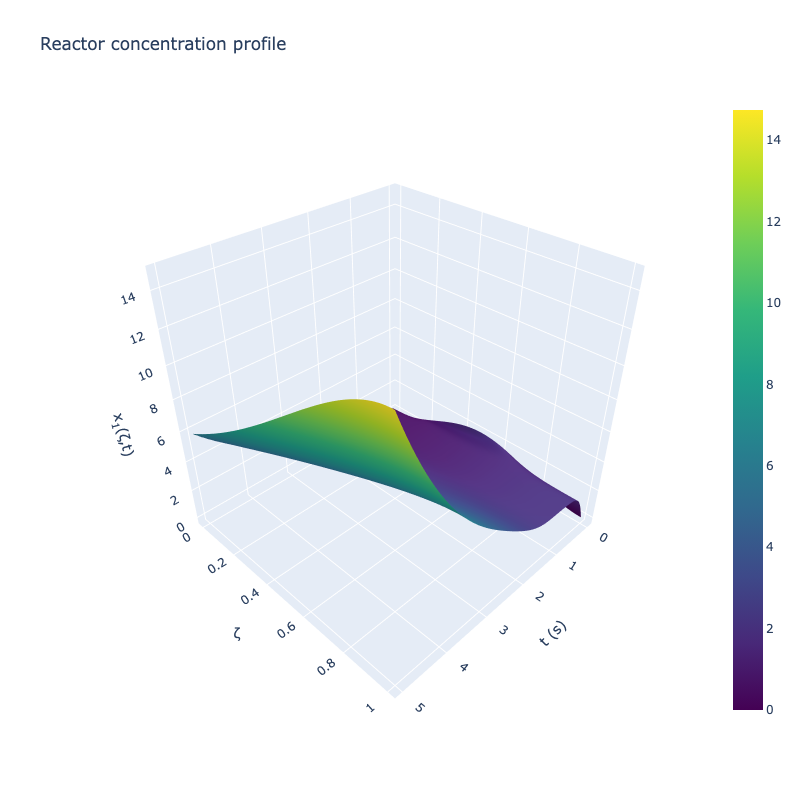
\includegraphics[width=0.8\textwidth,trim=0 0 100 0,clip]{Figures/3D_x1_openloop.png}
    \caption{Zero-input response of the unstable open-loop system as described by Equations~(\ref{eq:PDE_original_model})~and~(\ref{eq:BC}).}
    \label{fig:3D_x1_openloop}
\end{figure}

\subsection{Full-state feedback regulator FDM representation}


Next, the full-state feedback regulator is evaluated using the same FDM representation. Two configurations are compared where the optimal feedback gain is obtained using different number of eigenmodes: one with $N=3$ and another with $N=7$, according to Figure~\ref{fig:k_modes}. The state profile versus time and space is illustrated for both cases in Figure~\ref{fig:full_state_feedback}. 

\begin{figure}[!htbp]
    \centering
    \begin{subfigure}[b]{0.45\textwidth}
        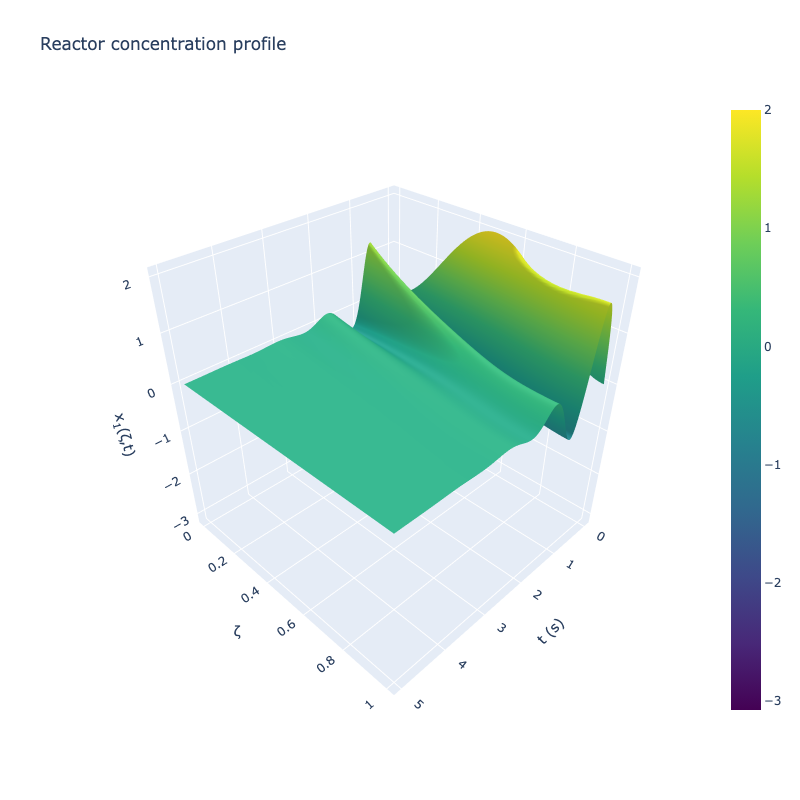
\includegraphics[width=\textwidth,trim=0 0 100 0,clip]{Figures/3D_x1_k3.png}
        \caption{$N=3$}
        \label{fig:3D_x1_k3}
    \end{subfigure}
    \hfill
    \begin{subfigure}[b]{0.45\textwidth}
        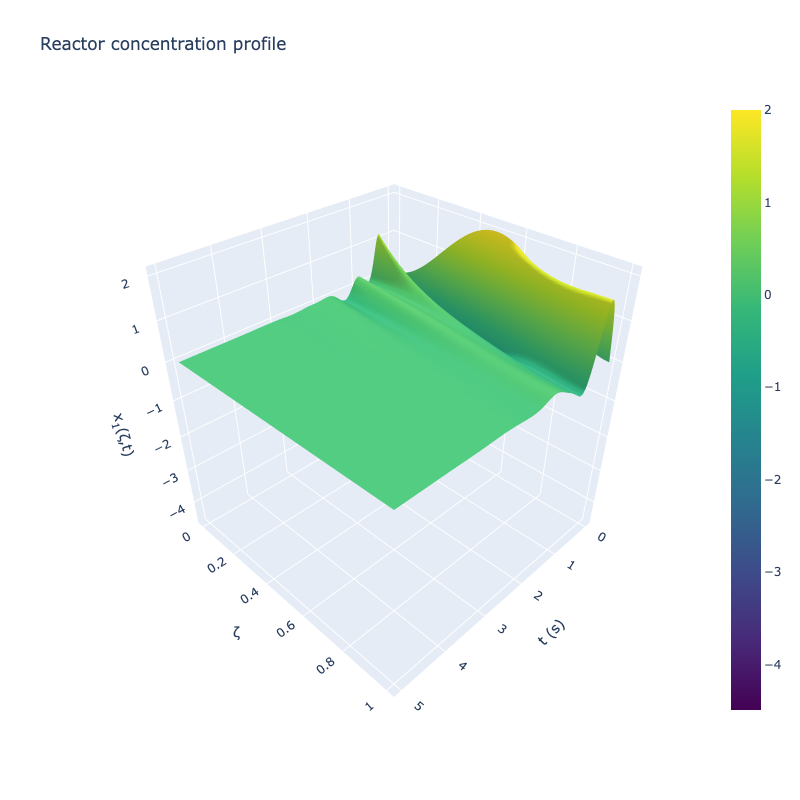
\includegraphics[width=\textwidth,trim=0 0 100 0,clip]{Figures/3D_x1_k7.png}
        \caption{$N=7$}
        \label{fig:3D_x1_k7}
    \end{subfigure}
    \caption{Input response of the system under full-state feedback control given by Equation~(\ref{eq:fullstate_ss}), utilizing the feedback gain obtained in Figure~\ref{fig:k_modes}.}
    \label{fig:full_state_feedback}
\end{figure}

Additionally, in order to offer a clearer representation of the state trajectory in time, spatial cross-sectional plots are provided in Figure~\ref{fig:2D_xt_k7} for the $N=7$ case at different lengths of the domain. The delay-imposing state, i.e. the concentration along the recycle stream $x_2(\zeta,t)$, is provided only in Figure~\ref{fig:2D_xt_k7} for the sake of conciseness.

\begin{figure}[!htbp]
    \centering
    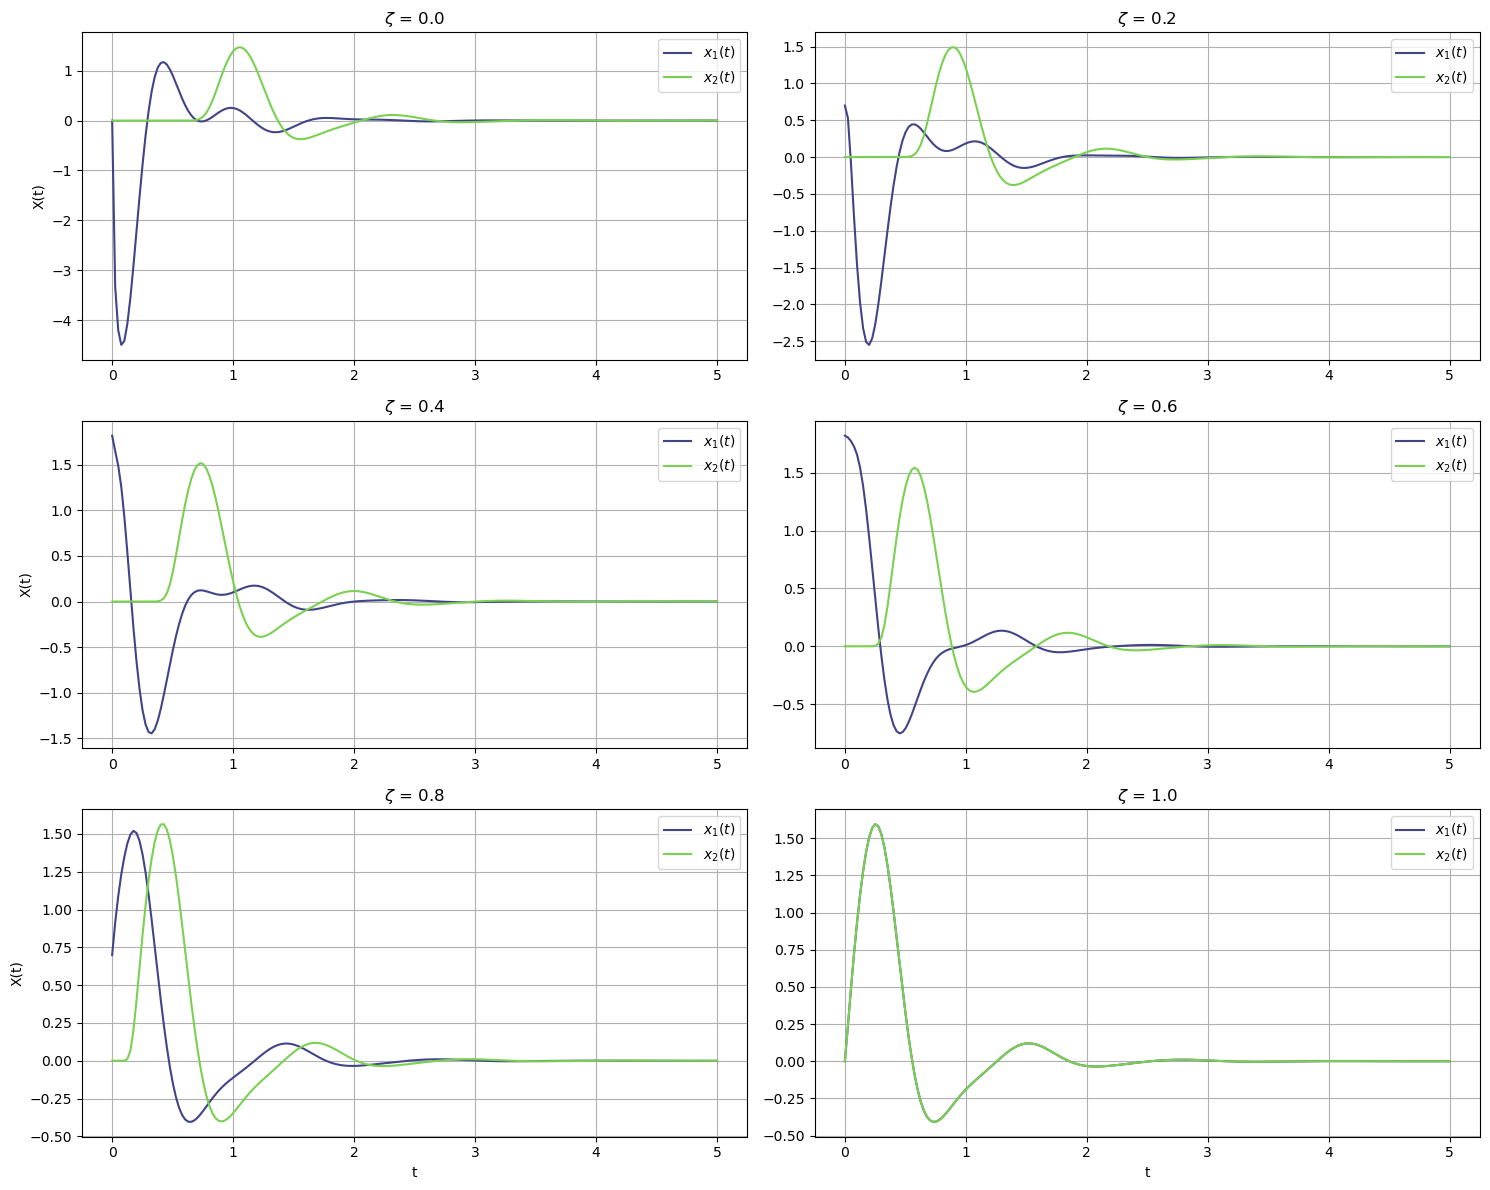
\includegraphics[width=0.8\textwidth]{Figures/2D_xt_k7.png}
    \caption{2D cross-section plots of the full-state feedback input response at various $\zeta$ positions, utilizing the feedback gain obtained in Figure~\ref{fig:k_7}.}
    \label{fig:2D_xt_k7}
\end{figure}

Both optimal feedback gains are able to successfully stabilize the system within finite time horizon. However, the case where more eigenmodes are considered in the controller design shows better performance in general. Sharing the same $\mathfrak{Q}$ and $\mathfrak{R}$ operators, the higher dimensional controller is able to stabilize the system quicker with lower cost function values in general.

\subsection{Observer-based regulator FDM representation}

Omitting the need to have full access to system states, the observer-based regulator is evaluated using the same FDM representation. The states reconstruction is done by applying the observer gain obtained in Figure~\ref{fig:L_modes} to the system output. The estimated states are now used with the previously obtained optimal feedback gain with $N=7$ eigenmodes to calculate the input. Similar to the previous case, the state profile $x_1(\zeta,t)$ is illustrated in Figure~\ref{fig:3D_x1_L_k7}, as well as cross-sectional plots for both states in Figure~\ref{fig:2D_xt_L_k7} for better visualization of state trajectories in time.

\begin{figure}[!htbp]
    \centering
    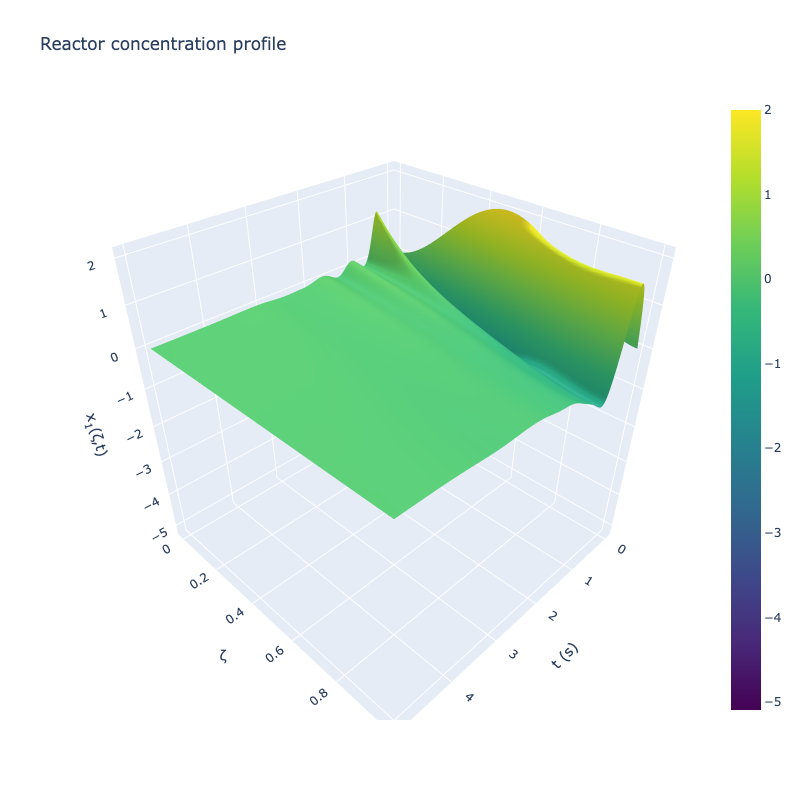
\includegraphics[width=0.8\textwidth,trim=0 0 100 0,clip]{Figures/3D_x1_L_k7.png}
    \caption{Input response of the system under observer-based output feedback control given by Equation~(\ref{eq:observer_ss}), utilizing the observer gain obtained in Figure~\ref{fig:L_modes} and the feedback gain obtained in Figure~\ref{fig:k_7}.}
    \label{fig:3D_x1_L_k7}
\end{figure}

\begin{figure}[!htbp]
    \centering
    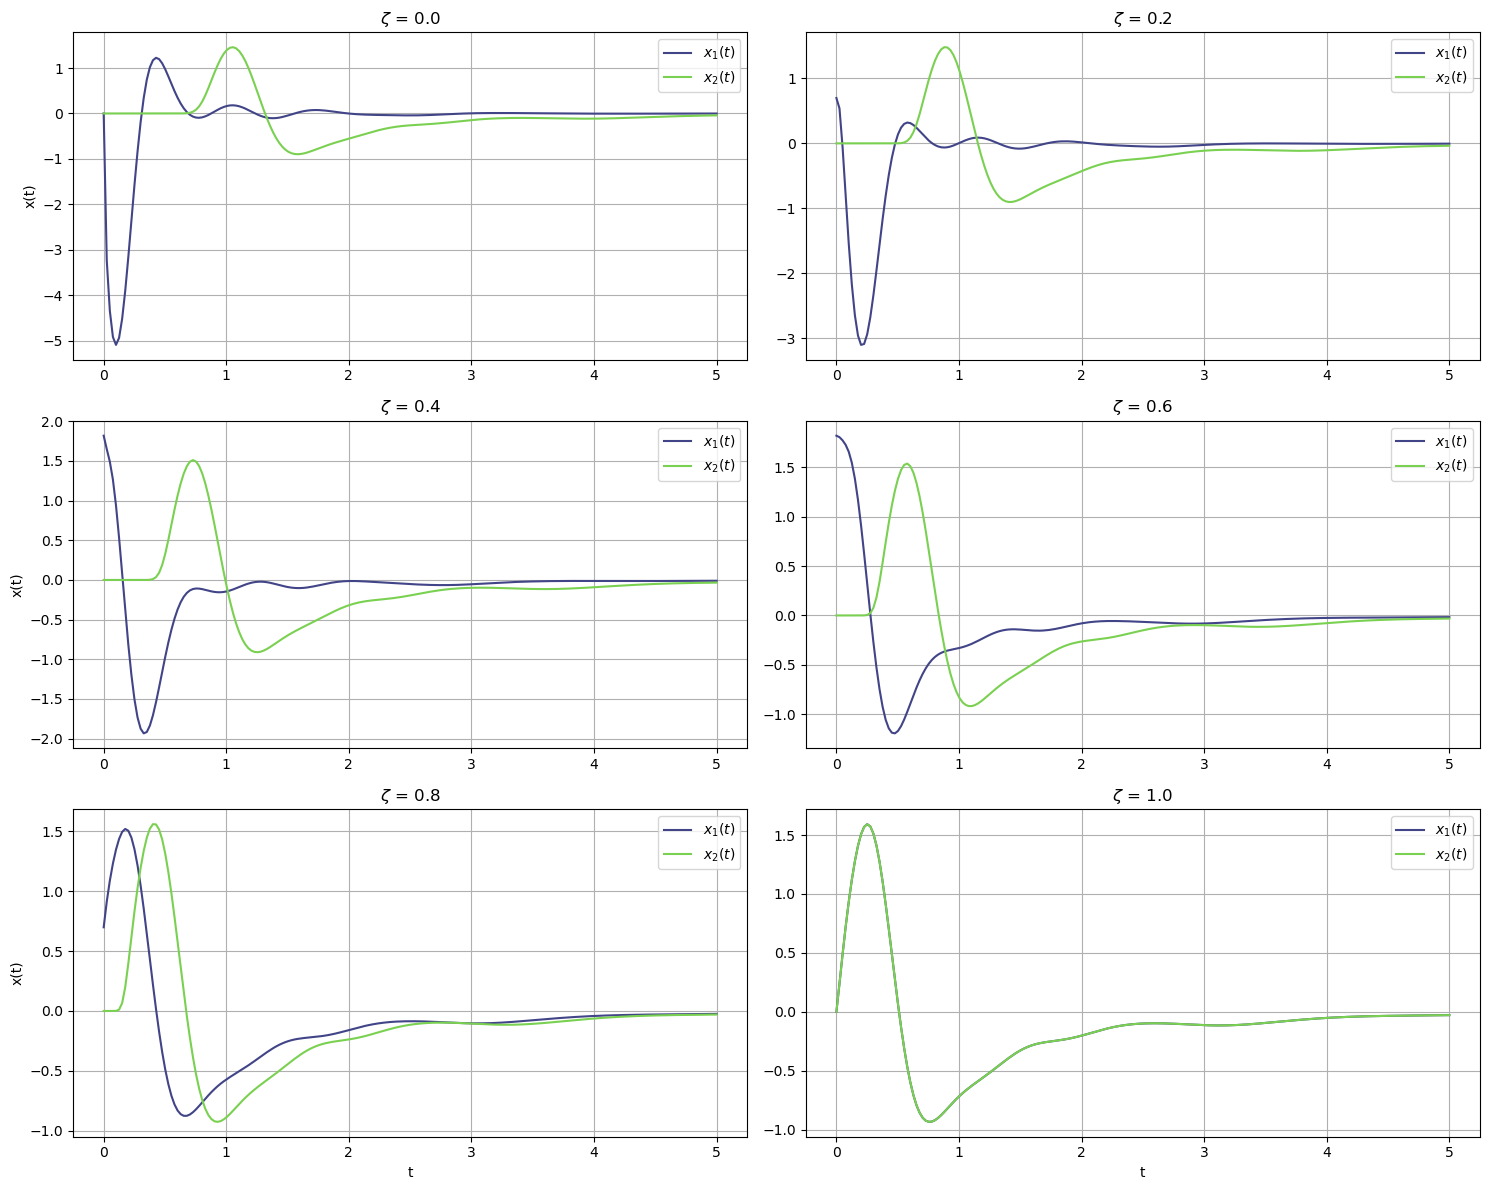
\includegraphics[width=0.8\textwidth]{Figures/2D_xt_L_k7.png}
    \caption{2D cross-section plots of the input response at various $\zeta$ positions, utilizing the observer gain obtained in Figure~\ref{fig:L_modes} and the feedback gain obtained in Figure~\ref{fig:k_7}.}
    \label{fig:2D_xt_L_k7}
\end{figure}

Last but not least, the state estimation error dynamics of the observer are plotted in Figures~\ref{fig:3D_e1_L_k7}~and~\ref{fig:2D_et_L_k7} to demonstrate the performance of the observer. The error dynamics are calculated as the squared difference between the true state and the estimated state at each grid point and time instance.

\begin{figure}[!htbp]
    \centering
    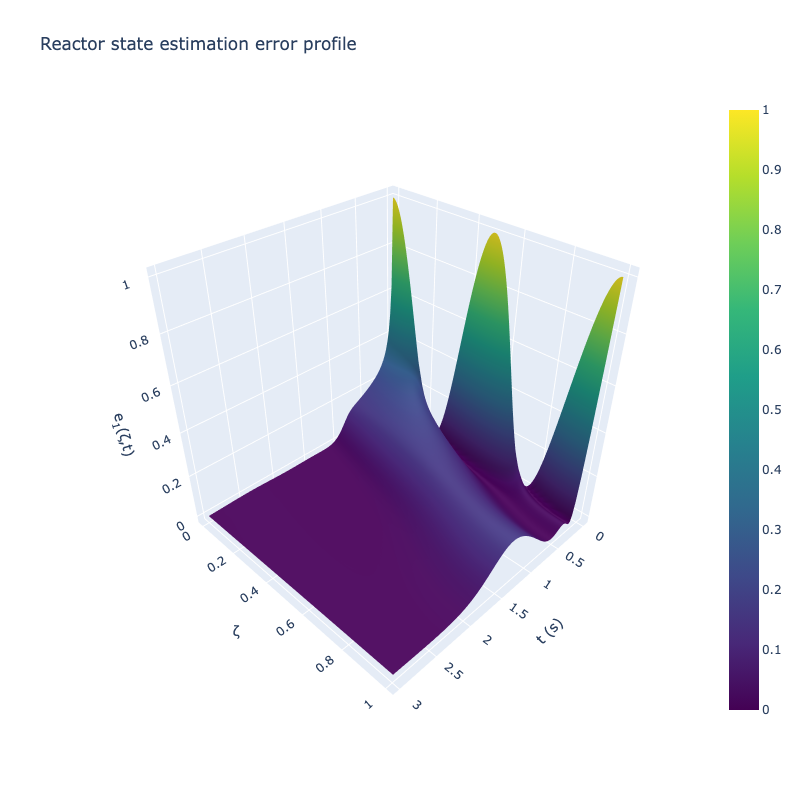
\includegraphics[width=0.8\textwidth,trim=0 0 100 0,clip]{Figures/3D_e1_L_k7.png}
    \caption{Error dynamics of the observer-based regulator utilizing the observer gain obtained in Figure~\ref{fig:L_modes} and the feedback gain obtained in Figure~\ref{fig:k_7}.}
    \label{fig:3D_e1_L_k7}
\end{figure}

\begin{figure}[!htbp]
    \centering
    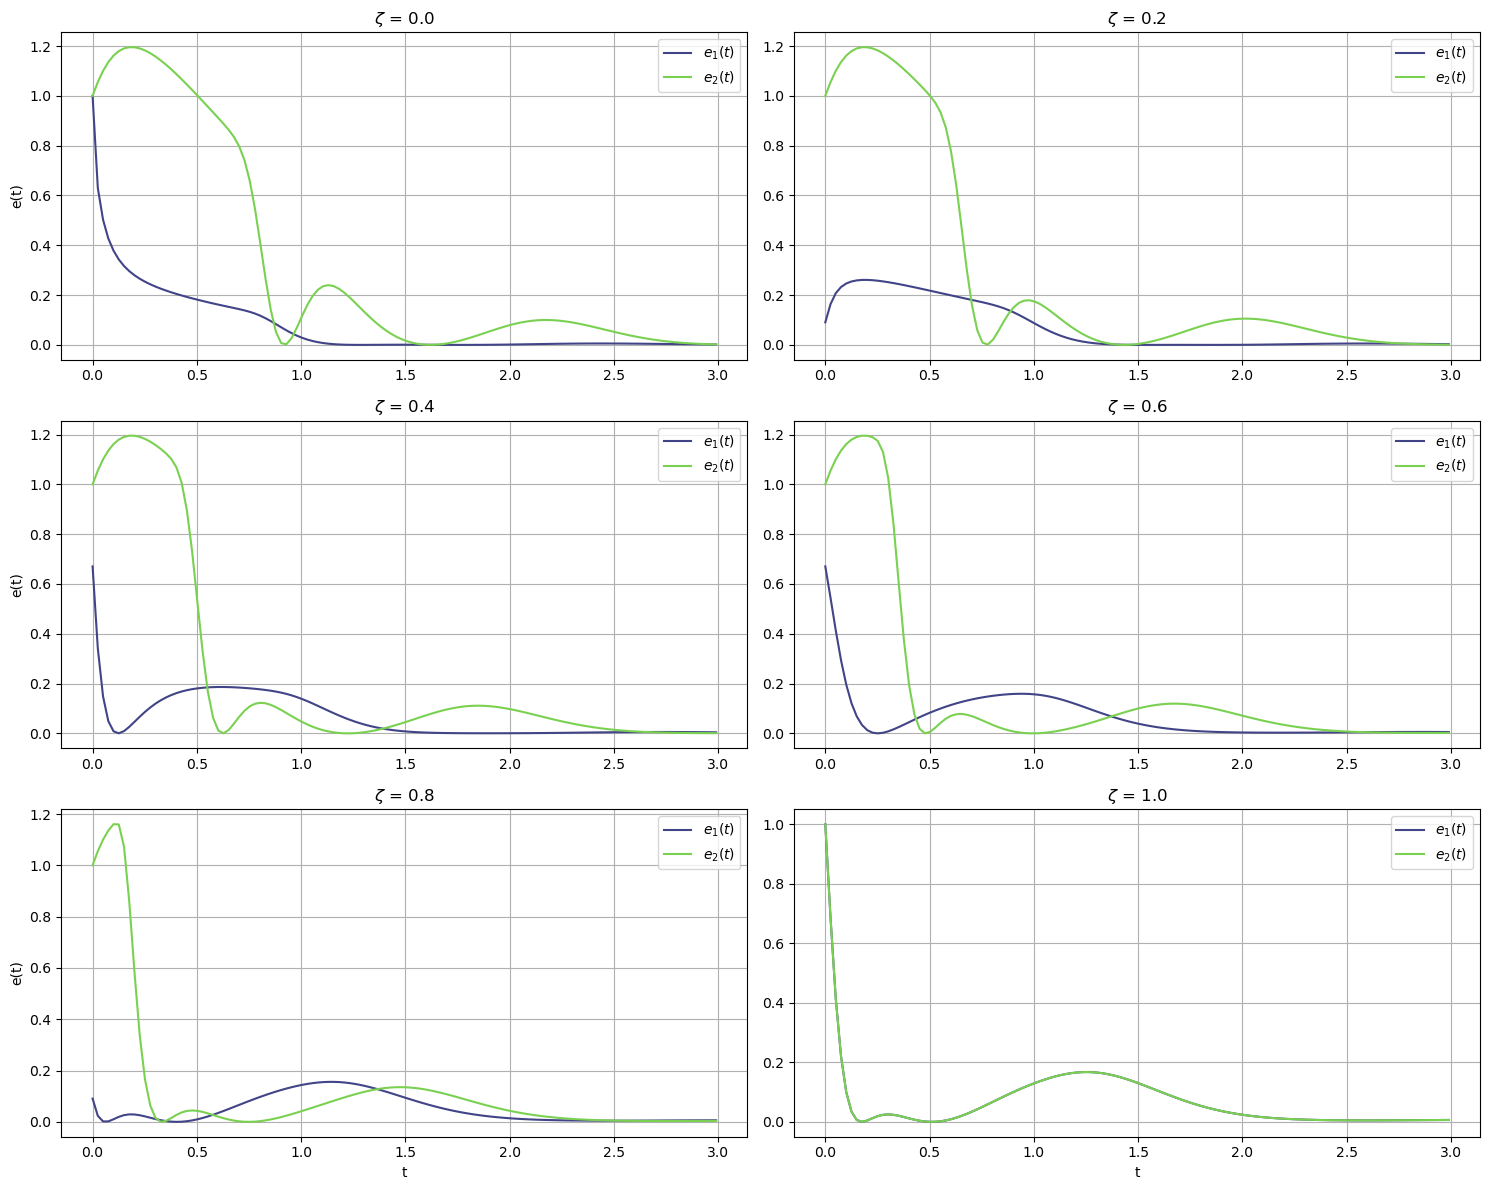
\includegraphics[width=0.8\textwidth]{Figures/2D_et_L_k7.png}
    \caption{2D cross-section plots of the error dynamics of the observer-based regulator at various $\zeta$ positions, utilizing the observer gain obtained in Figure~\ref{fig:L_modes} and the feedback gain obtained in Figure~\ref{fig:k_7}.}
    \label{fig:2D_et_L_k7}
\end{figure}

While the performance of the observer-based controller is slightly more sluggish compared to that of the full-state feedback regulator, it successfully stabilizes the system within a finite time horizon using only output measurements instead of full state information. In the absence of uncertainty in the system model, the observer gain can theoretically be designed so that the state estimation error converges to zero very fast compared to full-state feedback regulator dynamics. In practice, however, the observer gain is constrained by factors such as noise in the system output and plant-model mismatches. Despite these challenges, the proposed observer design mechanism achieves system stabilization with reasonable performance.